\section{The Extended Complex Numbers}

\begin{definition}
    We define the \textbf{extended complex numbers} to be the set $\C_\infty=\C
    \cup \{\infty\}$.
\end{definition}

\begin{lemma}\label{1.3.1}
    $\C_\infty$ is homeomorphic to the unit sphere $S^2$ of $\R^3$.
\end{lemma}
\begin{proof}
    Identify $\C$ with the plane $\R^2$ as a subset of $\R^3$. Then  $\C$ cuts
    the sphere  $S^2$ along the equator. Now, let  $N=(0,0,1)$ be the noth pole
    of $S^2$. For  $z \in \C$, let  $L_z$ the line passing through $z$ and $N$,
    and hence cuts  $S^3$ at exactly one point  $Z \neq N$. If  $|z|>1$,  $Z$
    is in the northern hemisphere of  $S^2$, and if  $|z|<1$, then  $Z$ is in
    the southern hemisphere. If  $|z|=1$, then  $Z=z$. Then notice that as
    $|z| \xrightarrow{} \infty$, then $Z \xrightarrow{} N$; and so identify
    $N$ with  $\infty$ in  $\C_\infty$.

    Now, let  $z=x+iy$ and  $Z=(x_1,x_2,x_3)$ a point on $S^2$. Then
    $L_z=\{tN+(1-t)z : t \in \R\}$. Observe then that
    \begin{equation*}
        L_z=\{((1-t)x,(1-t)y,t) : t \in \R\}
    \end{equation*}
    Then we get
    \begin{equation*}
        1=(1-t)^2|z|^2+t^2
    \end{equation*}
    Taking $t \neq 1$ so that  $z \neq \infty$
    \begin{equation*}
        Z=\Big{(}\frac{2x}{|z|^2+1},\frac{2y}{|z|^2+1},
        \frac{|z|^2-1}{|z|^2+1}\Big{)}
    \end{equation*}
    additionally
    \begin{equation*}
        Z=\Big{(}\frac{z+\bar{z}}{|z|^2+1},-i\frac{z-\bar{z}}{|z|^2+1},
        \frac{|z|^2-1}{|z|^2+1}\Big{)}
    \end{equation*}
    Taking $Z \neq N$ and  $t=x_1$, we also get by definition of $L_z$, that
    \begin{equation*}
        z=\frac{x_1+ix_2}{1-x_3}
    \end{equation*}

    Define now, the metric $d$ on  $\C_\infty$ by  $d(z,w)$ is the distance
    between the points $Z=(x_1,x_2,x_3)$ and $W=(y_1,y_2,y_3)$ on $S^2$. Then we
    get
    \begin{equation*}
        d(z,w)=\sqrt[]{(x_1-y_1)^2+(x_2-y_2)^2+(x_3-y_3)^2}
    \end{equation*}
    Squaring both sides we ovserve tha
    \begin{equation*}
        d(z,w)=2-2(x_1y_1+x_2y_2+x_3y_3)
    \end{equation*}
    Using the previous derivations of the components of $Z$, we finally obtain
    \begin{equation*}
        d(z,w)=\frac{z|z-w|}{\sqrt[]{(|z|^2+1)(|w|^2+1)}} \text{ for all }
        z,w \in \C
    \end{equation*}
    When $w=\infty$, we have
    \begin{equation*}
        d(z,\infty)=\frac{z}{\sqrt[]{|z|^2+1}}
    \end{equation*}
    Then $d$ is the required homeomorphism.
\end{proof}

\begin{figure}[h]
    \centering
    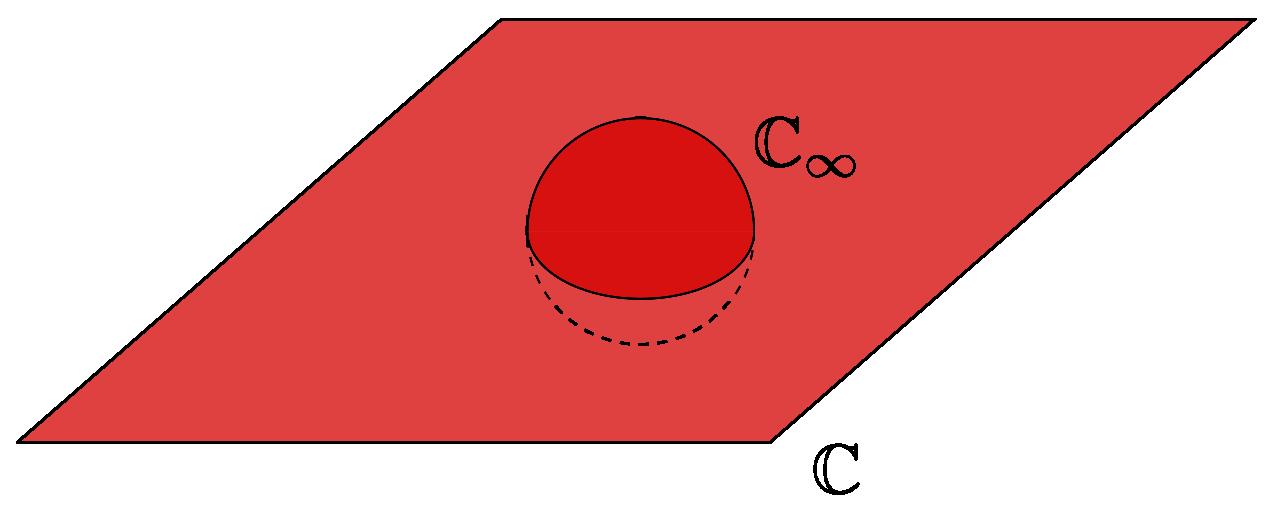
\includegraphics[scale=0.5]{Figures/chapter1/extended_complex_numbers.eps}
    \caption{The Extended Complex Numbers.}
    \label{fig_1.2}
\end{figure}

\begin{definition}
    We call the correspondence between $S^2$ and  $\C_\infty$ the
    \textbf{stereographic projection} of $S^2$ onto $\C_\infty$.
\end{definition}
